\section{杂项（Misc）安全}
\label{sec:misc}

\subsection{Misc 概述}
Misc（杂项）是 CTF 竞赛中覆盖范围最广、形式最灵活的题型，主要考察参赛人员的综合分析能力、编码解码能力、隐写分析能力、网络流量分析能力等。

\subsubsection{Misc 核心学习参考}
\begin{itemize}[leftmargin=*]
    \item CTF Wiki 杂项简介：\url{https://ctf-wiki.org/misc/introduction/}
    \item CTF之misc杂项解题技巧总结（一）——编码与加密：\url{https://blog.csdn.net/zjzqxzhj/article/details/128030485}
    \item CTF学习-MISC杂项解题思路：\url{https://blog.csdn.net/qq_44204058/article/details/119963204}
    \item Misc详细参考：\url{https://www.cnblogs.com/limestone/p/16869417.html}
\end{itemize}

\subsubsection{Misc 核心考察方向}
Misc 题目涉及知识面广泛，核心考点主要包括：
\begin{itemize}[leftmargin=*]
    \item 各类编码解码
    \item 隐写术分析
    \item 网络流量分析
    \item 压缩包分析与破解
    \item 系统日志分析
    \item 电子取证
    \item 信息收集与整理
    \item \textbf{PyJail 沙箱逃逸}（Python 代码执行限制绕过）
\end{itemize}

\subsection{Misc 常用工具介绍}
\begin{table}[htbp]
    \centering
    \caption{Misc 题型常用工具清单}
    \begin{tabular}{ll}
        \toprule
        工具名称 & 工具用途 \\
        \midrule
        WinHex / HxD / 010 Editor & 十六进制编辑器，用于文件底层结构分析 \\
        strings & Linux 命令，提取文件中的可打印字符串 \\
        binwalk & 检测并提取文件中隐藏的资源 \\
        foremost & 文件恢复与隐藏文件提取 \\
        file & Linux 命令，识别文件类型 \\
        StegSolve & 图片隐写分析工具，支持位平面与 LSB 分析 \\
        Photoshop & 图像编辑与隐写分析 \\
        Pillow & Python 图像处理库 \\
        PNGcheck & PNG 文件结构检测工具 \\
        Audacity & 音频处理与音频隐写分析 \\
        Wireshark & 网络流量数据包分析 \\
        ARCHPR & RAR/ZIP 压缩包密码破解 \\
        CyberChef & 在线编码解码与数据处理工具 \\
        330k Unicode Steganography & 零宽字符文本隐写解密 \\
        \bottomrule
    \end{tabular}
\end{table}

\subsubsection{CyberChef 工具详解}
CyberChef 是一款开源、跨平台、功能强大的在线数据处理工具，被称为“网络安全瑞士军刀”，支持各类编码、加密、哈希、格式转换等操作，是 CTF Misc 题型的高频使用工具。

在线地址：\url{https://gchq.github.io/CyberChef}

\begin{figure}[htbp]
    \centering
    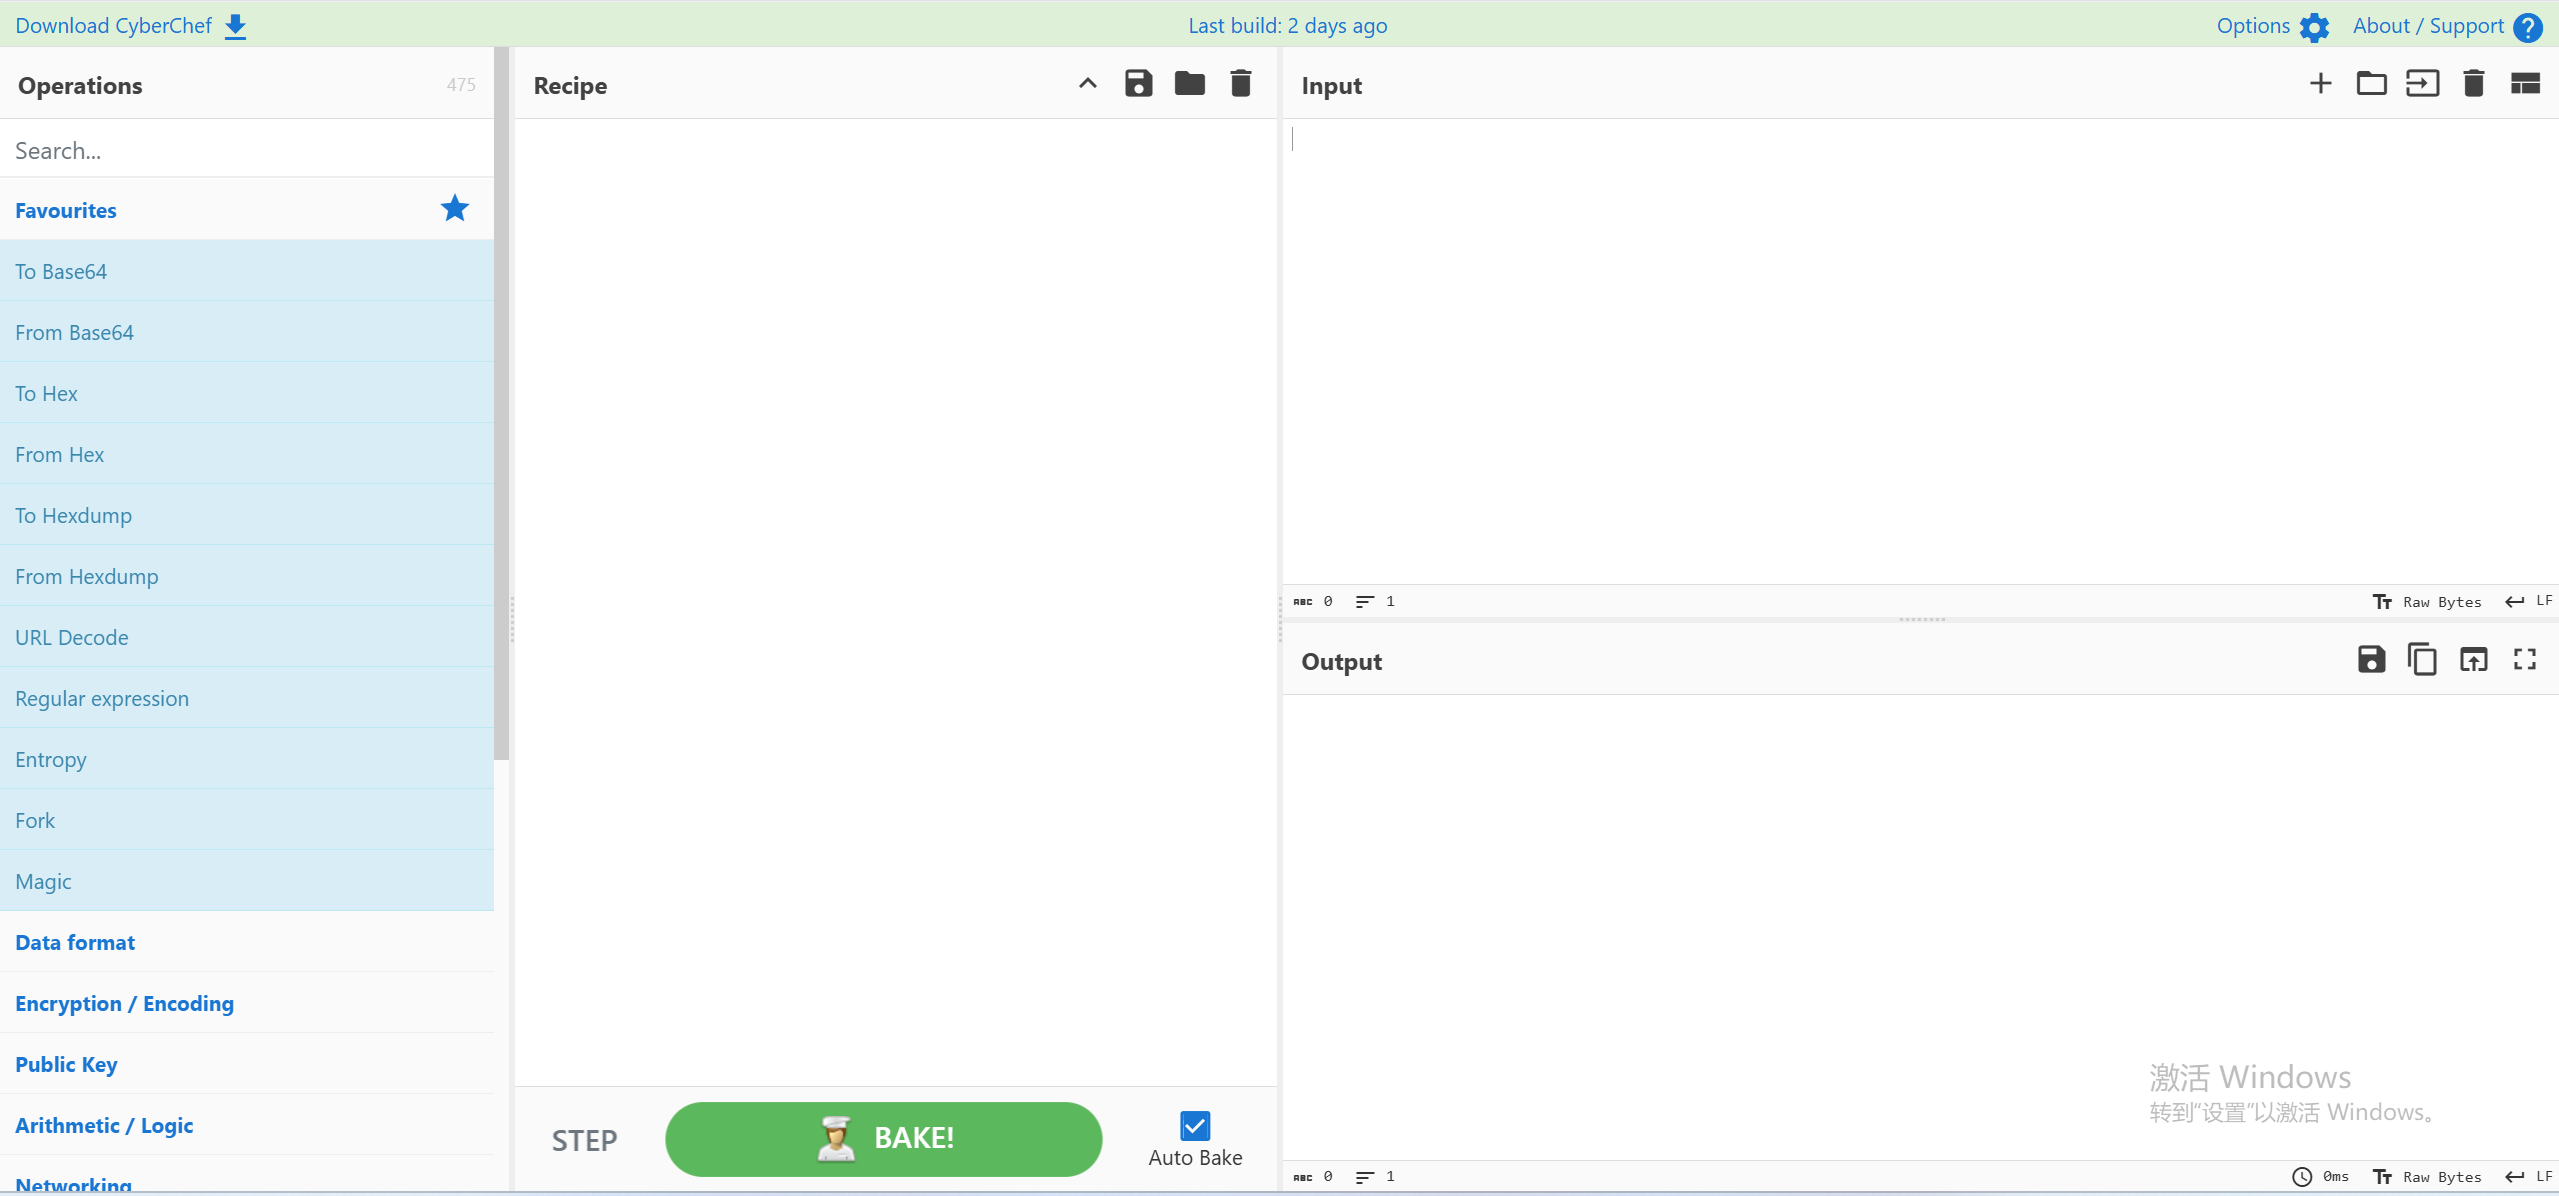
\includegraphics[width=0.9\textwidth]{4.1.png}
    \caption{CyberChef 工具界面与工作流程}
\end{figure}

工具使用流程：
\begin{enumerate}[leftmargin=*]
    \item \textbf{Input}：输入待处理数据
    \item \textbf{Operations}：选择需要的操作
    \item \textbf{Recipe}：组合多步处理操作
    \item \textbf{Output}：点击 BAKE! 获得结果
\end{enumerate}

\subsection{编码分析}
\subsubsection{常见编码方式}
CTF 中高频出现的编码类型：
\begin{itemize}[leftmargin=*]
    \item ASCII 编码
    \item Base64 / Base32 等 Base 系列编码
    \item 摩尔斯电码
    \item ROT 系列编码
    \item Unicode 编码（含连字、NFKC 标准化）
    \item URL 编码
\end{itemize}

参考资料：\url{https://ctf-wiki.org/misc/encode/computer/#base}

\subsubsection{编码载体与常见场景}
\begin{itemize}[leftmargin=*]
    \item \textbf{载体形式}：flag 通常以编码字符串形式隐藏
    \item \textbf{签到题}：直接给出多层嵌套编码
    \item \textbf{隐藏题}：编码内容藏于流量、图片等文件中，需先提取再解码
\end{itemize}

\subsubsection{Base 系列编码特征}
\textbf{Base64 编码特征：}
\begin{itemize}[leftmargin=*]
    \item 字符集：A–Z、a–z、0–9、+、/
    \item 结尾可能有填充符 =
\end{itemize}

\textbf{Base32 编码特征：}
\begin{itemize}[leftmargin=*]
    \item 字符集：A–Z、2–7
    \item 仅大写字母与数字，无 +/
    \item 结尾可能有填充符 =
\end{itemize}

\subsection{PyJail 沙箱逃逸例题：Truncate}
\subsubsection{题目源码与分析}
\begin{lstlisting}[language=Python]
#!/usr/bin/python3 -S
flag = open("flag.txt", "r").read().strip()
eval(input("")[:8])
\end{lstlisting}

\paragraph{代码解析}
\begin{itemize}[leftmargin=*]
    \item \texttt{-S}：禁用 site 模块，不影响本题核心逻辑
    \item 读取 flag.txt 内容存入变量 \texttt{flag}
    \item 获取用户输入，仅保留前 8 个字符，使用 \texttt{eval()} 执行
\end{itemize}

\paragraph{限制与目标}
\begin{itemize}[leftmargin=*]
    \item \textbf{限制}：输入长度最多 8 个字符
    \item \textbf{目标}：执行代码并泄露 \texttt{flag}
    \item \textbf{难点}：\texttt{print(flag)} 长度为 9，超出限制
\end{itemize}

\subsubsection{解题核心：Unicode 连字与 NFKC 标准化}
Python 在执行 \texttt{eval()} 前，会自动对字符串进行 NFKC 标准化。
部分 Unicode 连字字符会被展开为多个普通字符：
\begin{itemize}[leftmargin=*]
    \item \texttt{U+FB01} → \texttt{fi}
    \item \texttt{U+FB03} → \texttt{ffi}
    \item \texttt{U+FB00} → \texttt{ff}
\end{itemize}

利用该特性，可以实现**1 个字符输入 → 展开为多个字符**，从而突破长度限制。

\subsubsection{Payload 构造}
构造 Payload：
\[
\texttt{U+FB01 (flag)}
\]
经过 NFKC 标准化后变为：
\[
\texttt{int(flag)}
\]
长度仅 6 个字符，符合 8 字符限制，可成功执行并输出 flag。

\subsubsection{环境连接与执行}
\begin{itemize}[leftmargin=*]
    \item 环境：SEEDUbuntu 虚拟机
    \item 连接命令：\texttt{nc <IP> <Port>}
    \item 输入 Payload：\texttt{int(flag)} 获取 flag
\end{itemize}

\subsection{隐写术（Steganography）}
\label{subsec:misc_steganography_full}

\subsubsection{隐写术概述}
隐写术是将秘密信息隐藏在图片、音频、视频、文本、压缩包等载体中，实现隐蔽传输的技术，是 CTF Misc 中的核心考点。

\paragraph{CTF 中隐写术的常见特点}
\begin{itemize}[leftmargin=*]
    \item 题目多以文件附件形式给出，文件可能无后缀，需先识别文件类型
    \item 隐写术常与混淆、编码、密码学相结合，需多层分析才能提取 flag
\end{itemize}

\paragraph{常见载体}
\begin{itemize}[leftmargin=*]
    \item 图片（PNG、BMP）
    \item 音频（WAV、MP3）
    \item 文本（零宽字符隐写）
    \item 压缩包（伪加密、文件合并）
\end{itemize}

\subsubsection{文件识别基础}
\paragraph{文件识别方法}
\begin{itemize}[leftmargin=*]
    \item \textbf{后缀名识别}：通过文件后缀初步判断类型（不可靠，可伪造）
    \item \textbf{工具识别}：使用 \texttt{file} 命令（Linux）、\texttt{010 Editor} 等工具分析
    \item \textbf{文件头识别}：通过文件开头的魔数（Magic Number）精准识别文件类型（最可靠）
\end{itemize}

\paragraph{常见文件头对照表}
\begin{table}[htbp]
    \centering
    \caption{CTF 常见文件类型与对应文件头}
    \begin{tabular}{ll}
        \toprule
        文件类型 & 文件头（十六进制） \\
        \midrule
        JPEG (jpg) & FFD8FFE1 \\
        PNG (png) & 89504E47 \\
        GIF (gif) & 47494638 \\
        TIFF (tif) & 49492A00 \\
        Windows Bitmap (bmp) & 424DC001 \\
        ZIP Archive (zip) & 504B0304 \\
        RAR Archive (rar) & 52617221 \\
        Adobe Photoshop (psd) & 38425053 \\
        Rich Text Format (rtf) & 7B5C727466 \\
        XML (xml) & 3C3F786D6C \\
        HTML (html) & 68746D6C3E \\
        Adobe Acrobat (pdf) & 255044462D312E \\
        Wave (wav) & 57415645 \\
        pcap (pcap) & 4D3C2B1A \\
        \bottomrule
    \end{tabular}
\end{table}

\paragraph{文件操作常用工具}
\begin{itemize}[leftmargin=*]
    \item \textbf{判断文件类型}：\texttt{file}（Linux 命令）
    \item \textbf{查看/修改文件}：\texttt{WinHex}、\texttt{010 Editor}、\texttt{notepad++}、\texttt{Hex Editor}
    \item \textbf{分离文件}：\texttt{binwalk}、\texttt{foremost}、\texttt{dd}
    \item \textbf{文件检测/处理}：\texttt{Stegsolve}、\texttt{Pillow}
    \item \textbf{文件合并}：\texttt{cat}（Linux）、\texttt{copy}（Windows）
\end{itemize}

\subsubsection{图像隐写（LSB 隐写详解）}
\paragraph{LSB 隐写核心原理}
LSB（Least Significant Bit，最低有效位）是一种常见的信息隐藏方法。
图像像素一般由 RGB 三原色组成，每一种颜色占 8 位（\texttt{0x00~0xFF}，即 256 种颜色），而人的肉眼能区分的只有其中一小部分。

LSB 隐写就是修改 RGB 颜色分量中最低的二进制位：
\begin{itemize}[leftmargin=*]
    \item 仅修改像素中最低的 1 bit，肉眼完全无法区分前后变化
    \item 每个像素可携带 3 bit 信息（RGB 三通道各 1 bit）
    \item 不影响图片正常显示，同时隐藏秘密信息（通常为 \texttt{flag{xxx}} 格式）
\end{itemize}

\paragraph{StegSolve 实操步骤（图像隐写例题）}
\begin{enumerate}[leftmargin=*]
    \item 打开 StegSolve，加载目标图片
    \item 点击 \texttt{Analyse} → \texttt{Data Extract}
    \item 位平面设置：仅勾选 \textbf{Red 0、Green 0、Blue 0}（最低有效位）
    \item 字节序设置：选择 \texttt{LSB First}，\texttt{Bit Order} 选择 \texttt{RGB}
    \item 点击 \texttt{Preview} 查看隐藏数据，提取 flag 相关内容
\end{enumerate}

\subsubsection{音频隐写（摩斯码隐写详解）}
\paragraph{音频隐写核心原理}
音频隐写利用人耳对声音的不敏感特性，将秘密信息（如摩斯码）隐藏在音频文件中，通过分析音频波形提取信息。

\paragraph{工具：Audacity 实操步骤}
\begin{enumerate}[leftmargin=*]
    \item 打开 Audacity，加载音频文件 \texttt{secret.wav}
    \item 观察音频波形，识别有节奏的滴答声，对应摩斯码的点（·）和划（-）
    \item 提取摩斯码序列
    \item 使用在线摩斯码转换工具解码，得到 flag
\end{enumerate}

\paragraph{自动音频摩斯密码解码工具（无需看波形、无需听）}
\begin{itemize}[leftmargin=*]
    \item 在线音频摩斯自动解码：\url{https://morsecode.world/international/decoder/audio-decoder-adaptive.html}
    \item 功能：直接上传音频文件，自动识别摩斯密码并输出明文
    \item 适用场景：CTF 音频隐写（滴答声类型摩斯密码）
\end{itemize}

\paragraph{摩斯码隐写核心考点}
\begin{itemize}[leftmargin=*]
    \item 摩斯码基础：点（·）、划（-）、间隔（字符间隔/单词间隔）
    \item 音频波形分析：通过波形长短区分点和划
    \item 在线解码工具：快速将摩斯码转换为明文 flag
\end{itemize}

\subsubsection{文本隐写}
文本隐写利用不可见字符实现信息隐藏，典型为**零宽字符隐写**，将秘密信息编码进 Unicode 零宽字符中并嵌入普通文本，肉眼无法察觉。

\paragraph{常见零宽字符}
\begin{itemize}[leftmargin=*]
    \item 零宽空格（U+200B）
    \item 零宽连接符（U+200D）
    \item 零宽非连接符（U+200C）
\end{itemize}

\paragraph{分析工具与步骤}
\begin{itemize}[leftmargin=*]
    \item Sublime Text / VSCode：显示不可见字符，提取零宽字符序列
    \item 330k 官方零宽隐写工具：\url{http://330k.github.io/misc_tools/unicode_steganography.html}
    \item 备用在线工具：\url{https://www.mzy0.com/ctftools/zerowidth1/}
\end{itemize}

\paragraph{标准解题流程}
\begin{enumerate}[leftmargin=*]
    \item 将含隐写的文本粘贴至 330k 零宽字符隐写工具
    \item 点击 Decode 按钮直接提取隐藏信息
    \item 对解码结果进行整理，得到最终 flag
\end{enumerate}

\subsubsection{隐写术通用解题思路}
\begin{enumerate}[leftmargin=*]
    \item \textbf{文件类型识别}：用 \texttt{file}/\texttt{010 Editor} 识别载体，补全后缀
    \item \textbf{载体针对性分析}：
    \begin{itemize}[leftmargin=*]
        \item 图片：StegSolve 位平面与 LSB 提取
        \item 音频：Audacity 波形分析与摩斯码提取
        \item 文本：零宽字符提取与解码
        \item 压缩包：binwalk 提取并逐层解压
    \end{itemize}
    \item \textbf{编码/密码学处理}：对提取的信息进行解码、解密
    \item \textbf{按正则构造 flag 并提交}
\end{enumerate}

\subsection{隐写术常用工具汇总}
\begin{table}[htbp]
    \centering
    \caption{隐写术全载体常用工具清单}
    \begin{tabular}{ll}
        \toprule
        工具名称 & 工具用途 \\
        \midrule
        StegSolve / StegOnline & 图片位平面分析、LSB 提取、PNG 块分析 \\
        Audacity & 音频处理、摩斯码提取与分析 \\
        010 Editor & 16 进制编辑、文件头识别 \\
        Sublime Text & 零宽字符查看 \\
        330k Unicode Steganography & 零宽字符文本隐写解密 \\
        CyberChef & 编码解码、LSB 提取 \\
        binwalk & 隐藏文件提取 \\
        7-Zip / WinRAR & 压缩包解压 \\
        \bottomrule
    \end{tabular}
\end{table}

\subsection{网络安全竞赛通用工具清单}
\begin{table}[htbp]
    \centering
    \caption{网络安全竞赛全题型常用工具}
    \begin{tabular}{ll}
        \toprule
        工具类别 & 代表工具 \\
        \midrule
        渗透测试 & Burp Suite、Nmap、Metasploit \\
        逆向分析 & IDA Pro、Ghidra、x64dbg \\
        密码学 & CyberChef、John the Ripper、Hashcat \\
        取证分析 & Wireshark、Volatility、Foremost \\
        \bottomrule
    \end{tabular}
\end{table}

\subsection{参考文献}
\begin{enumerate}[leftmargin=*]
    \item 《CTF那些事儿》，李舟军，机械工业出版社，2023
    \item 《CTF特训营：技术详解、解题方法与竞赛技巧》，FlappPig战队著，机械工业出版社，2022
    \item 《CTF竞赛权威指南（Pwn篇）》，杨超，电子工业出版社，2020
    \item 《白帽子Web安全》，吴翰清，电子工业出版社，2021
    \item 《CTF安全竞赛入门》，张镇等，清华大学出版社，2020
    \item Unicode 标准与规范化形式：\url{https://unicode.org/reports/tr15/}
    \item Python eval 与 Unicode 标准化：\url{https://docs.python.org/3/reference/lexical_analysis.html#unicode-normalization}
    \item 摩斯码在线转换工具：\url{http://mosi.fjnews.com/}
    \item 音频摩斯密码自动解码工具：\url{https://morsecode.world/international/decoder/audio-decoder-adaptive.html}
    \item 零宽字符隐写工具：\url{http://330k.github.io/misc_tools/unicode_steganography.html}
\end{enumerate}